\section{Baterías de ion-litio}

A finales del año 2019, año en el que se comenzó esta tesis, la Real Academia 
de Ciencias de Suecia le otorgó el Premio Nobel en Química a J. B. Goodenough, 
M. S. Whittingham y A. Yoshino por sus contribuciones al desarrollo de la batería 
de ion-litio. Esta batería recargable permitió los avances que se vieron en los 
teléfonos móviles y en las computadoras portátiles, entre otras aplicaciones.
Además, permite un mundo libre de combustibles fósiles ya que se utiliza en 
vehículos eléctricos y en almacenamientos estacionarios de energía para fuentes
renovables. Este galardón restaltó la importancia de muchos aspectos de la ciencia
moderna, como la investigación básica, la investigación la aplicada, la 
interdisciplina (JBG fue físico, MSW es un químico y AY un ingeniero) los 
desarrollos tecnológicos y los problemas concretos de las sociedades.
En la década del 1970, MSW desarrolló la primera batería utilizando un ánodo de
litio metálico y un cátodo de disulfuro de titanio. En 1980, JBG duplicó el 
voltaje original de dicha batería al introducir un cátodo de óxido de cobalto.
La desventaja de ambas se encontraba en el ánodo de litio metálico, que en los 
ciclos de carga y descarga se deposita preferentemente en sitios donde ya se 
ha depositado, dando lugar a estructuras ramificadas, llamadas dendritas, que 
pueden cortocircuitar la celda y llevar a la explosión de la misma. En 1985,
AY remplazó este material por uno carbonoso que incorpora los iones de litio
durante la carga y la descarga, disminuyendo los riesgos mencionados. Basandose
en este desarrolló, Sony comenzó a comercializar baterías de ion-litio en 1991.
La densidad de energía de estas baterías rondaba los 80 Wh/kg, en la actualidad
WeLion comercializa para los EVs de Nio una batería de ion-litio con una 
densidad de energía de 360 Wh/kg. En la Figura \ref{fig:whkg} se muestra la 
evolución de la densidad de energía en baterías de ion-litio comercializadas 
en los últimos 30 años. La importancia de esta característica para los EVs 
radica en la relación autonomía/peso.

\begin{figure}[h!]
    \centering
    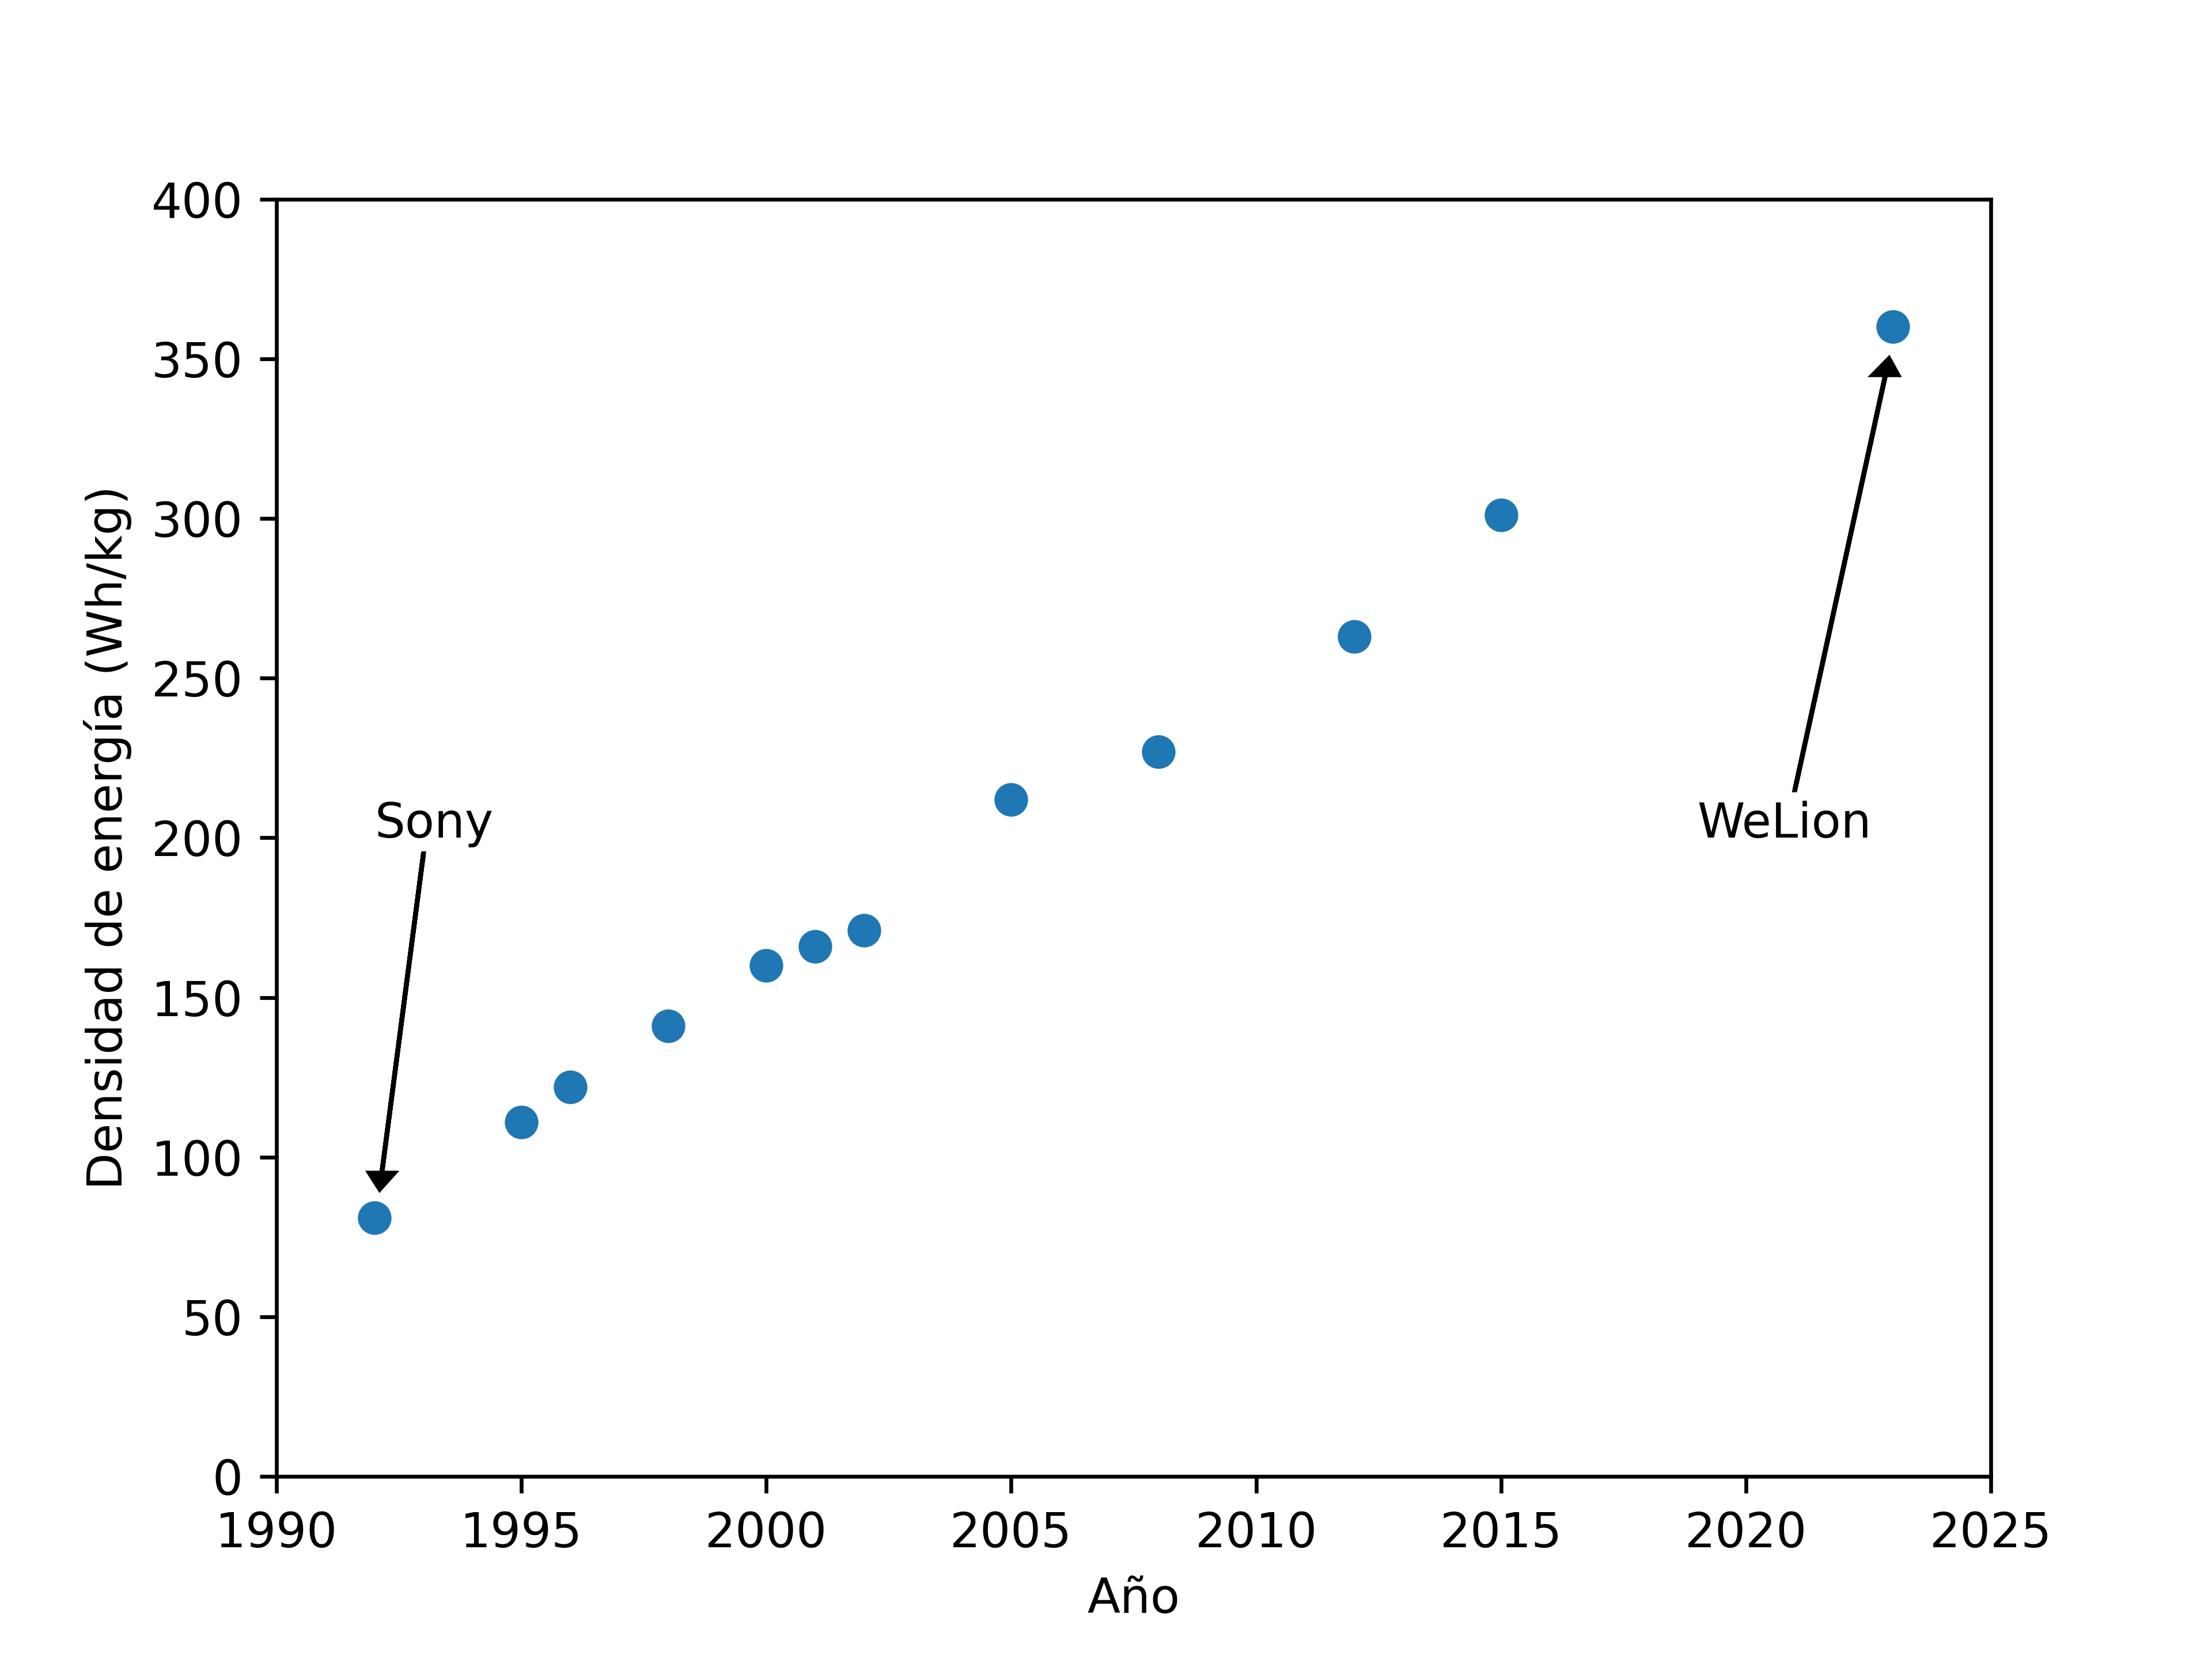
\includegraphics[width=.8\textwidth]{Introduccion/baterias/whkg.png}
    \caption{Aumento en la densidad de energía en baterías de ion-litio comercializadas
    en los últimos 30 años. Figura adaptada de \cite{li2023700}.}
    \label{fig:whkg}
\end{figure}

\begin{figure}[h!]
    \centering
    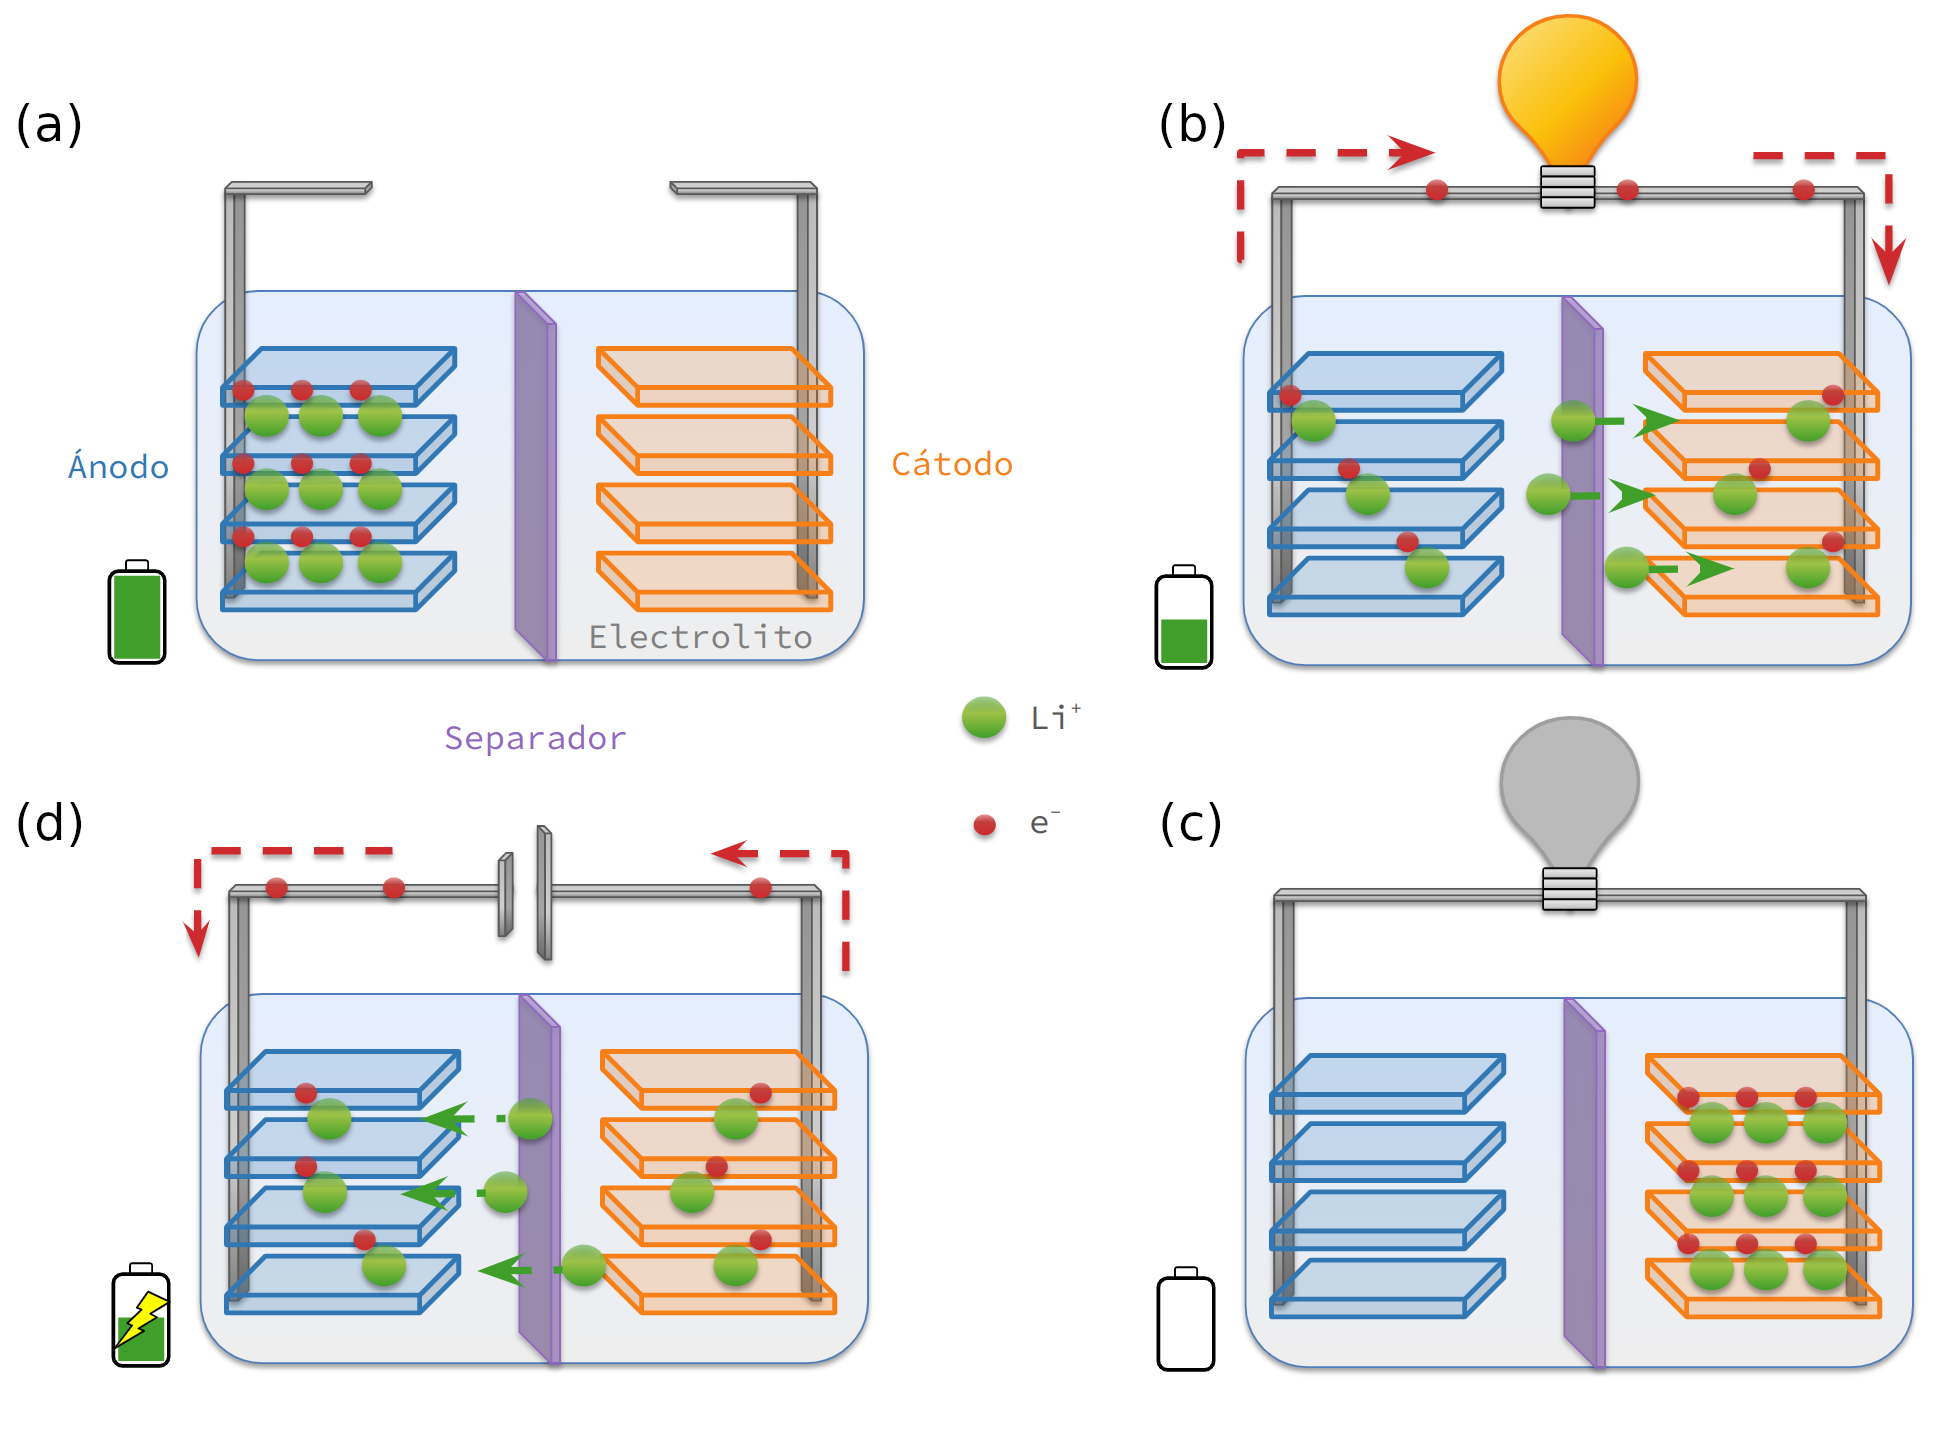
\includegraphics[width=.8\textwidth]{Introduccion/baterias/esquema_bateria.png}
    \caption{Esquema de las componentes y el funcionamiento de una batería de 
    ion-litio.}
    \label{fig:esquema-bateria}
\end{figure}

En la Figura \ref{fig:scopus} se muestra el incremento en las últimas dos décadas
de los artículos científicos publicados en el área de las baterías de litio y, en 
particular, de las dos ramas estudiadas en esta tesis: la Carga rápida y los 
Ánodos de Si. En dicha figura se presentan datos extraídos de la base de datos 
Scopus \cite{SCOPUS} del número de publicaciones anuales normalizado con respecto 
al número de publicaciones en el año 2003, año en el que hubo 710 publicaciones 
en baterías de litio, 32 sobre ánodos de Si y 0 sobre carga rápida, por lo que 
se normalizó en este caso a la única publicación del 2004 en el tema.
\begin{figure}[h!]
    \centering
    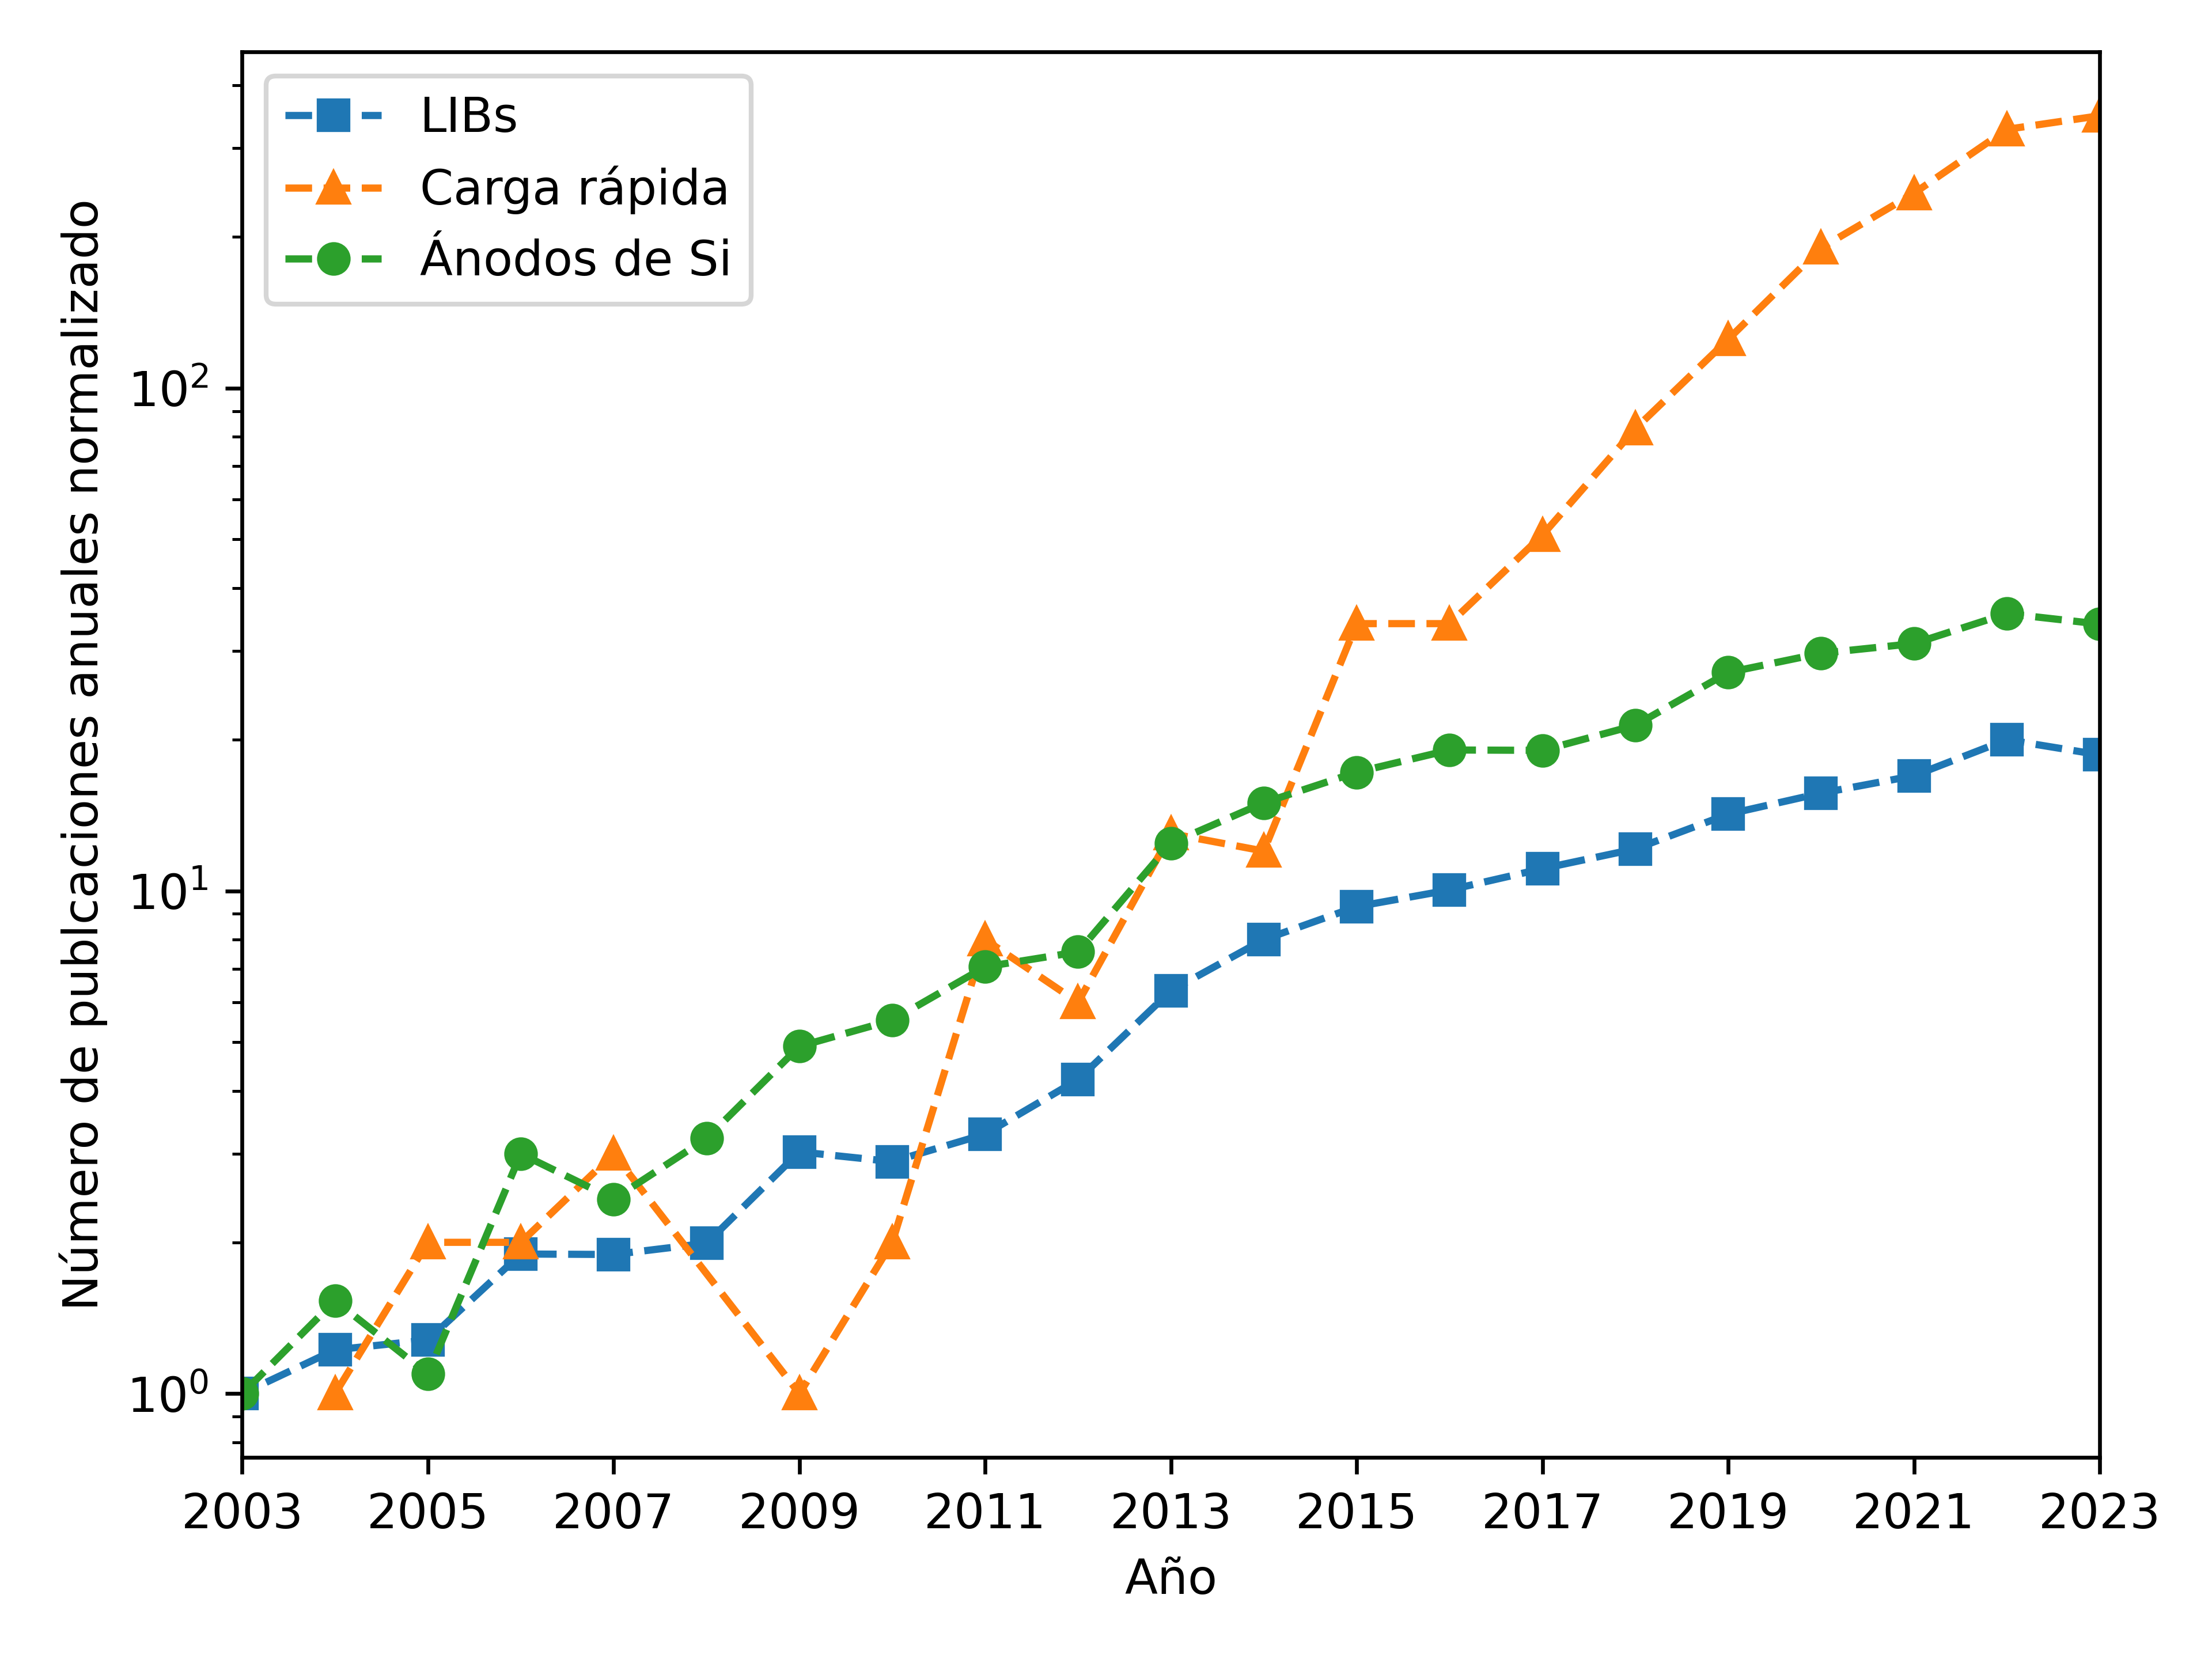
\includegraphics[width=.8\textwidth]{Introduccion/baterias/scopus.png}
    \caption{Número de publicaciones anuales normalizado con respecto al año 2003. 
    Las consultas realizadas en Scopus \cite{SCOPUS} incluyen: 
    \texttt{lithium AND battery} (LIBs, en azul), \texttt{lithium AND battery AND 
    fast-charging} (Carga rápida, en naranja) y \texttt{lithium AND battery AND 
    silicon anodes} (Ánodos de Si, en verde).}
    \label{fig:scopus}
\end{figure}
La normalización y la escala logarítmica en la Figura \ref{fig:scopus} permiten
observar cualitativamente que la pendiente de crecimiento de publicaciones 
realcionadas a la carga rápida de baterías de litio es considerablemente mayor a 
de las otras dos. Además, los ánodos de Si se encuentran dentro de lo que sería
el creciemiento promedio del área de las baterías de litio. Un análisis de datos
cuantitativo permite determinar que en la última década el aumento de porcentaje
anual de publicaciones promedio fue del 15 \% y 16 \% para las baterías de litio 
y para los ánodos de silicio, respectivamente, mientras que para la carga rápida 
este porcentaje promedio asciende al 52 \%. Este análisis demuestra la relevancia
que la comunidad científica le da a los temas estudiados en esta tesis.
